\documentclass[oneside,12pt]{book}

% Package dependencies
\usepackage{geometry}
\usepackage{lipsum}
\geometry{left=32mm, right=30mm, bottom=25mm, top=25mm}
\usepackage{amsmath , amsthm , amssymb}
\usepackage{float}
\usepackage{hyperref}
\usepackage{apacite}
\usepackage{scrextend}
\usepackage{blindtext}
\usepackage{fancyhdr}
\usepackage{multicol}
\usepackage{csquotes}
\usepackage{bm}
\usepackage{subcaption}
\usepackage{tocbibind}
\usepackage{pdfpages}
\usepackage[toc,page]{appendix}
\usepackage{wrapfig}
\usepackage{colortbl}
\usepackage{multirow}
\usepackage{listings}

% document formatting
\addtokomafont{labelinglabel}{\sffamily}
\setlength{\columnsep}{1cm}
\renewcommand{\baselinestretch}{1.5}


\begin{document}

% Title page
\begin{titlepage}
    \begin{center}
        \vspace*{1.5cm}
        \Huge
        \textbf{Performance comparison between a distributed particle swarm algorithm and a non distributed algorithm}
        
        \vspace{0.5cm}
        \begin{figure}[H]
    	\centering
    	\hspace{7mm} \includegraphics[scale=0.5]{TU_logo}
        \end{figure}
        
        \vspace{1.5cm}
        
        \textbf{Ciarán O'Loughlin}
        
        \vfill
       \large
        A dissertation submitted in partial fulfilment of the requirements of\\
	Dublin Institute of Technology for the degree of\\
	M.Sc. in Computing (TU060)\\
       \vspace{0.5cm}
        \textbf{Date}
        \vspace{0.8cm}
 
    \end{center}
\end{titlepage}

% Define headers / footer style for the whole doc
\pagestyle{fancy}
\fancyhf{}
\fancyfoot[CE,CO]{\thepage}
\renewcommand{\headrulewidth}{0pt}

% APA style for referencing
\bibliographystyle{apacite}

% Roman numerals for the 'administrative' sections
\pagenumbering{Roman}

% Declaration page
\chapter*{Declaration}
\addcontentsline{toc}{chapter}{Declaration}
I certify that this dissertation which I now submit for examination for the award of
MSc in Computing (Stream), is entirely my own work and has not been taken
from the work of others save and to the extent that such work has been cited and
acknowledged within the text of my work.
\\
\\
This dissertation was prepared according to the regulations for postgraduate study of
the Dublin Institute of Technology and has not been submitted in whole or part for an
award in any other Institute or University.
\\
\\
The work reported on in this dissertation conforms to the principles and requirements
of the Institute’s guidelines for ethics in research.
\vfill
\noindent
\textit{\textbf{Signed:}}  \\

\noindent
\textit{\textbf{Date:}}
\vspace{0.8cm}

% Abstract
\chapter*{Abstract}
\addcontentsline{toc}{chapter}{Abstract}
\par 

\vfill
\noindent
\textbf{Keywords:} \quad Swarm Intelligence, Particle Swarm Optimisation, PSO, Distributed Algorithms

%Acknowledgements
\chapter*{Acknowledgments}
\addcontentsline{toc}{chapter}{Acknowledgments}

% Contents and lists
\newpage
\tableofcontents

\listoffigures

\listoftables

\chapter*{List of Acronyms}
\addcontentsline{toc}{chapter}{List of Acronyms}
\begin{table}[H]
  \centering
    \begin{tabular}{ l l }
    \textbf{PSO} & Particle Swarm Algorithm \\
    \textbf{LTS} & Long Term Support \\
    \textbf{CPU} & Computer processor unit \\
    \textbf{RAM} & Random Access Memory \\
    \end{tabular}
\end{table}

\newpage

% Standard numbering starts from here
\pagenumbering{arabic}
\fancyhead[RE,LO]{\leftmark}
\renewcommand{\headrulewidth}{2pt}


% Start of core thesis content

%Introduction chapter
% ============================================================= %
\chapter{Introduction}
\section{Background}
\par Swarm Intelligence (SI) is an innovative distributed intelligent paradigm for solving optimization problems that originally took its inspiration from the biological examples by swarming, flocking and herding phenomena in vertebrates \cite{abraham_guo_liu_2006}.
Within the boundaries of swarm intelligence there are many different algorithms, all with different uses and capabilities. One particular algorithm is the Particle swarm optimisation algorithm(PSO). PSO is a population-based search algorithm and is initialized with a population of random solutions, called particles \cite{shi_2004}. Particles are then arranged into a "swarm". Swarms allow the sharing of information between particles, the so called "social" element of the algorithm. Particle swarm optimisation as an algorithm was first proposed by James Kennedy  and Russell Eberhart in their 1995 paper "Particle Swarm Optimization" \cite{kennedy_eberhart_1995}. While not a new technique, PSO is still being expanded upon today, with modern uses ranging from simple algorithmic evaluation, to more complex robotics implementations. 

This is the basis of a single swarm PSO. We can increase the number of particles in a swarm, but we can also increase the number of swarms. A multi swarm PSO(Or a Cooperative Particle Swarm Optimisation algorithm, CPSO) model allows for "a significant increases in the solution diversity in CPSO-S algorithm, because of the many different members from different swarms" \cite{vandenbergh_engelbrecht_2004}. Even when using a multi swarm model, there will be hard limits on the number of particles and swarms a singular machine can generate. This is where a distributed model can help, with swarms being logically segregated across a network of machines.

\section{Research Project/problem}
There is an upper limit to the amount of particles any one system can support in a PSO algorithm. At a certain point the algorithm will slow down and the time taken for it to complete an iteration will drastically increase. This will be exacerbated by running multiple swarms. 
To alleviate this problem we can distribute the swarms onto different machines, which allows us to increase the total number of swarms and particles available to us. However, this has a disadvantage as to evaluate results generated by the swarms network communications will need to be established. Network connections are inherently slower than connections and data transfers on a local machine, so the question this report aims to answers is

\textit{"At what point are performance gains in running a particle swarm optimisation algorithm in a distributed environment outweighed by the time lost in network communications between multiple swarms?"}

\section{Research Objectives}
The key objective  of  the  research  is  to  identify  whether  there exists a point whereby its more efficient to run a particle swarm optimisation algorithm in a distributed manner over a non distributed manner. To answer this question the following research objectives where identified:
\begin{enumerate}
\item Create a distributed and non distributed implementation of the PSO
\item Generate a result set for the non distributed implementation, with varying inputs(Example; different evaluation function, number of swarms and or particles etc.). Average out results with the same inputs
\item Generate a result set for the distributed implementation, with varying inputs(Examples; different evaluation function, number of swarms and or particles etc.). Average out results with the same inputs
\item Cross comparison between the two results sets. Identify points at which distributed had a faster response time, or other values that would make it preferable to  a non distributed implementation
\item Identify any limiting factors, significant points of interest in the data and identify future research
\end{enumerate}


\section{Research Methodologies}
The research can be classified based in a few different ways -
\subsection{Based on Type: Primary vs Secondary}
Primary research refers to a collection of original data, specific to a particular research question generated during the project. When doing primary research, the researcher gathers information first-hand rather than relying on available information in databases and other publications.\cite{bouchrika_2020}

Secondary research instead focus's on collecting and summarizing existing data collections and results. This involves researching existing literature, published articles and analyzing the data produced from these articles to come to a new conclusion, or test a hypothesis. When doing secondary research, researchers use and analyze data from primary research sources.\cite{bouchrika_2020}

The research type for this project can be defined as primary research. Data sets needed to answer the research question will be generated during the course of the project. The data set will be unique, as no other study has sought to compare implementation types of particle swarm optimisation algorithms. 
\subsection{Based on Objective: Quantitative vs Qualitative}
Quantitative research methods refer to collecting numerical data, data that can be used to measure variables, predict outcomes etc. Quantitative data is structured and statistical, using a grounded theory method that relies on data collection that is systematically analyzed. Quantitative research is a methodology that provides support when you need to draw general conclusions from your research and predict outcomes.\cite{mcleod_2019}

Qualitative research is the fundamentally opposite to Quantitative research, as it relies on non-statistical and unstructured or semi-structured. It is a methodology designed to collect non-numerical data to gain insights. It relies on data collected based on a research design that answers the question “why.”\cite{survey_monkey}

The research objective of this project can be defined as quantitative research. This study will generate and examine structured data sets, comparing two particle swarm optimisation implementations, and drawing conclusions from those comparisons. 
\subsection{Based on Form: Exploratory vs Constructive vs Empirical}
Exploratory research refers to when researching a problem which has not been clearly defined. Through exploratory research we can determine the best research design and data collection method. 
When conducting constructive research a completely new approach, theory or model will be proposed. Constructive research adds a new contribution to the current body of research. 
Empirical research is a way of obtaining knowledge through direct observation or experience. Empirical research involves a process, of defining a hypothesis, and then making predictions that can be tested using a suitable scientific experiment. The study can be defined as an empirical study. This study will define its hypothesis, test that hypothesis, examine the results from tests, and draw conclusions/predictions from the data. Based on that data the hypothesis can then be accepted or rejected, concluding the study.  

\subsection{Based on Reasoning: Deductive vs Inductive}
% Needs rewriting. :(
Deductive reasoning is a basic form of valid reasoning. Deductive reasoning, or deduction, starts out with a general statement, or hypothesis, and examines the possibilities to reach a specific, logical conclusion
Inductive reasoning is the opposite of deductive reasoning. Inductive reasoning makes broad generalizations from specific observations. Basically, there is data, then conclusions are drawn from the data. 

For this study deductive reasoning will be used. The study will state a hypothesis, and attempt to validate that hypothesis testing, generating data sets and drawing conclusions from those data sets. 

\section{Scope and Limitations}
The scope of this research is to identifier potential points where a distributed implementation of the particle swarm optimisation algorithm is faster than a centralised implementation. 

There are two main limiting factors to this research. The first being that the implementations are only tested against specific fitness functions. There are many different fitness functions that can be applied to a particle swarm optimisation algorithm, and many of them will have different efficiency points, some may gain a benefit from being distributed at different levels of swarms and particles, and others may not ever benefit from being distributed. For this reason four different algorithms where chosen and tested against the two implementations. 

The second limiting factor is an environmental one. Computers with a higher amount of CPU(Computer processor unit) power and RAM(Random Access Memory) will be able to support more swarms and particles. In order to account for this the same machine type will be used across the distributed and non distributed implementations. How this will be achieved is discussed in chapter three, Design and Implementation Overview. 

\section{Document Outline}
%Needs Rewritting, just place holder
\subsection{Chapter 1}
Chapter 1 is a short introduction and few reasons why this research was conducted.
\subsection{Chapter 2}
Chapter 2 involves a comprehensive literature review, including existing, similar approaches  to  solving the discussed issue using both architectural paradigms. Some gaps in the existing research  are discussed
\subsection{Chapter 3}
Chapter 3 includes a detailed design of the experiment as well as the methodology behind it.The execution of performance tests is also discussed.
\subsection{Chapter 4}
Chapter 4 contains some of the implementation details related to the performed benchmark. It also contains an valuation and discussion of gathered metrics and compiled results including plenty of metric graphs
\subsection{Chapter 5}
Chapter 5 is a final discussion and conclusion of the research project, including future suggestions on the given problem as well as recommendations regarding accuracy of the experiment and its design

% Literature review chapter
% ============================================================= %
\chapter{Background Research}
\section{Introduction}
This  chapter  provides  a  review of the  literature available on particle swarm optimisation algorithms, distributed implementation, various  approaches adopted  to  solve  the  problem  and  evaluation metrics used  for  evaluating  the results.  The  chapter  concludes with  the  gaps  in  the existing research and forms the objective for the research.
\section{PSO(Particle Swarm Optimisation)}
\subsection{What is PSO?}
The original PSO algorithm was introduced in 1995 \cite{kennedy1995particle}, in the paper they discussed what the PSO algorithm is, and how to use it to optimise nonlinear functions. At its heart PSO is a population based optimization technique where the population is referred to as a swarm, and population members are referred to as particles. At the algorithms inception, a number of unique particles are created and given random positions within a D-dimensional space. Each particle can be considered a potential solution to the fitness function. Particles then go through iterations, or epochs, where each particle calculates its own personal best evaluation value, then the global best value is calculated. Particles are encouraged to move closer to their own personal best or the groups based on the algorithms implementation. A particle moving closer towards the groups best will define a higher "social value", and moving closer to its own personal best will define a higher "cognitive value". Velocity can also be changed to reduce the variance in particle positions between iterations, also know as epochs. 
\begin{figure}[H]
    \centering
    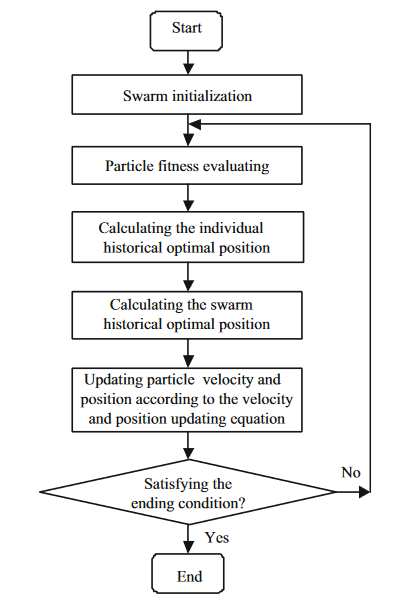
\includegraphics[scale=0.6]{Images/PSO_Flow.png}
    \caption{Flow Diagram of Particle Swarm Optimisation Algorithm \protect\cite{wang_tan_liu_2017}}
    \label{fig:Flow Diagram of Particle Swarm Optimisation Algorithm}
\end{figure}

We can see from the above explanation that PSO shares many elements of other artificial intelligence types, such as evolutionary computation, and genetic algorithms. The particles are manipulated according to the following equations: 
\begin{equation}
V_{id} = W * V_{id} + C_l * Rand( ) * ( P_{id} - X_{id} ) + C_2 * Rand( ) * (P_{gd} - X_{id})
\end{equation}
\begin{equation}
X_{id} = X_{id} + V_{id}
\end{equation}
Where Cl and c2 are two positive constants, Rand() is a random function in the range [0,1], and w is the inertia weight \cite{shi1998parameter}. A particle's new velocity can be calculated using equation 2.1, using its previous velocity and the distances of its current position from its own best experience (position) and the group's best experience. Equation 2.2 calculates the particles new position after its updated velocity. 

\subsubsection{Fitness Function}
When talking about PSO we must also talk about a fitness function. A fitness function is a function that maps the values in your particles to a real value that must reward those particle that are close to your optimisation criterion. Essentially this is the optimisation function you wish to find the minimum value. For instance if we wished to find the global minimum of the Beale Function, and optimisation test function we could use PSO. Beale function can be defined as:
\begin{equation}
f(x, y) = (1.5-x+xy)^2+(2.25-x+xy^2)^2+(2.625-x+xy^3)^2
\end{equation}
Using this fitness function we could find the global minimum, in this case it would equate out to be $f(x*)=0$ at $x*=(3,0.5)$ \cite{bingham}. Its important to note that as PSO is a heuristic algorithm, its solution results are not necessarily optimal. PSO will find an answer to a fitness function, but it may not be the best answer to the function. In addition, some problems may have multiple global minimum values, in which case the PSO can only find one answer at a time.


\section{PSO Implementations}
Since James Kennedy and Russell Eberhart original paper there has been significant research into the original algorithm \cite{piotrowski_napiorkowski_piotrowska_2020, bai_2010, imrantextordfeminine2013overview, wang_tan_liu_2017} its applications \cite{hereford_2006, beni_2005, blum_li, raquel2005effective} and its performance \cite{yin_yu_wang_wang_2006, kennedy_1999}. There is also a large body of research into the use of swarm algorithms in distributed environments \cite{akat_gazi_2008, salza_ferrucci_2019, peleg_2005} and centralised environments \cite{trelea_2003, xie2003overview, poli2007particle}, which will be discussed more in the following section. PSO has also been improved upon, with some newer implementations updating the topology or some other underlying principle of the algorithm, examples including SPSO, APSO, TRIBES, Cyber Swarm etc \cite{zhou2009gpu, oca_stutzle_birattari_dorigo_2009, cooren2009performance, yin2010cyber}.

In terms of implementing PSO there have been multiple studies into the uses of swarm intelligence in robotics system \cite{sa_nedjah_mourelle_2016, meng_gan_2008, hereford_2006}. Some other studies also look at interesting use cases PSO and swarm intelligence can be applied to, such as scheduling systems and analysis of distributed systems \cite{li_yang_su_lu_yu_2019, moradi_fotuhi-firuzabad_2008, nouiri_bekrar_jemai_niar_ammari_2015, sahin2007fault}. 

\subsection{Stopping Criteria}

\subsection{Parameter Selection}
As mentioned in earlier sections, there are multiple input parameters for any pso algorithm, the basic ones being inertia, cognitive and social weightings. Parameters are usually tuned for individual optimisation functions, but there are some basic selecting parameters that are normally used. 

\subsection{Topology adjustments}
Since its original inception, several adjustments have been proposed in literature to alter some implementation detail around PSO. One reaccuring change is a change to the population topology or sociometry. It is well established that these factors play an important role in improving the performance of population-based optimization algorithms by enhancing population diversity when solving multiobjective and multimodal problems \cite{LYNN201824}. Global version PSO (GPSO) and local version PSO (LPSO) are two common neighbor topologies. 
\subsubsection{G-PSO}
In  the  gbest  population,  the trajectory  of  each  particle’s  search  is  influenced  by  the best point found by any member of the entire population\cite{kennedy2002population}. What this means is that the particle uses its experience (the best position achieved so far), and uses the knowledge of the best particle in the swarm to influence its movement strategy. It prioritises the global best value when updating its position.  However, the drawback of this approach is that if the best particles is far  from global optimum, the  swarm can  be  trapped in  local optima since the swarm cannot explore other areas in the search space \cite{azab_hady_hefny_2016}

\subsubsection{L-PSO}
The  lbest  population  allows  each  individual  to  be  influenced  by  some  smaller  number  of  adjacent  members  of the  population  array. Typically  lbest  neighborhoods comprise exactly two neighbors, one on each side: a ring lattice.\cite{kennedy2002population}. The same update function is used by particles in the two topologies, however lbest is generally considered to be the slower topology. Its advantage though is that it's much less likely to get stuck in the local optima, and therefore finds the target value more frequently. 

\begin{figure}[H]
    \centering
    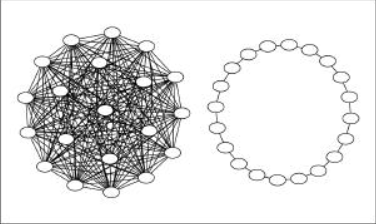
\includegraphics[scale=1.0]{Images/NeighborhoodTopology.png}
    \caption{GBest(Left) and LBest(Right) sociometric patterns.\protect\cite{kennedy2002population}}
    \label{fig:GBest(Left) and LBest(Right) sociometric patterns.}
\end{figure}

\subsection{Multi Swarm PSO}
As mentioned previously there has been a wide body of research conducted into variants of the original PSO algorithm. One such area has been in using multiple swarms, with researches finding some success with their implementations. One such implementation is the MSPSO(multi-swarm particle swarm optimization).  MSPO "\textit{is based on multiple swarms framework cooperating with the dynamic sub-swarm number strategy (DNS), sub-swarm regrouping strategy (SRS), and purposeful detecting strategy (PDS)}" \cite{XIA2018126}. Using these strategies allows MSPSO to balance its exploration and the exploitation ability, resulting in good performance, in terms of solutions accuracy. It however does suffer from an increased time complexity when compared to several other PSO implementations. 
IPSO(Improved  particle  swarm  optimization   algorithm) is another mutli swarm technique that "\textit{adopts   a   new   mutation  operator  and  a  new  method  that  congregates  some  neighboring  individuals  to  form  multiple  sub-populations  in  order  to  lead  particles  to  explore  new  search space}" \cite{zheng2007improved}. Subdividing out the population into multiple neighborhoods, or swarms allows the algorithm to divide up the problem space, and thereby improve performance. Utilising the mutation factor also allowed the implementation to "\textit{enhance the efficiency of advantageous direction of flying particles, so particles can fly to feasible region more quickly and more efficiently}".
\begin{figure}[H]
    \centering
    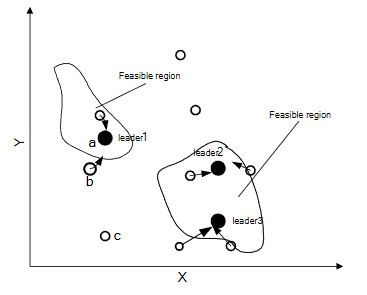
\includegraphics[scale=1.0]{Images/IpsoFormingSwarms.png}
    \caption{IPSO multi-populations being formed .\protect\cite{zheng2007improved} }
    \label{fig:IPSO multi-populations being formed.}
\end{figure}

\subsection{Distributed PSO}
\subsubsection{dPSO}
As mentioned in chapter one, there will be a limit to the number of particles and swarms any one computer can support, the limiting factor being the amount of memory or computational power. To avoid this bottle neck there has been a significant body of research into creating a distributed implementation of the PSO algorithm.  One such area of research is in robotics, using PSO as a search algorithm distributed across many particles, in reality acting as particles in the PSO. In James M. Hereford paper, "\textit{A Distributed Particle Swarm Optimization Algorithm for Swarm Robotic Applications}" a distributed PSO algorithm is proposed, which he calls the dPSO \cite{hereford_2006}. Listing 2.1 shows the pseudo code used to implement the algorithm. 

\begin{lstlisting}[language=inform, caption=Herefords dPSO Code Flow]
pbest = -1; gbest = -1; % Initialize pbest and gbest 
While (target not found or time not expired) 
	% Make measurement and update, if necessary 
    meas = make_measurement();  
    if (meas > pbest) % Update pbest, if true
    	Up_pbest(); %Update pbest value and location
        if (meas > gbest) % Update gbest, if true
        	Set gflag; % set a flag 
            Up_gbest(); %Update gbest value and location
        end 
     end 
     Move(); % Move bot based on PSO update equation  
     % For simulation, constrain bot movement 
     % Two conditions: 
     %   (1) Magnitude of velocity must be < Vmax 
     %   (2) Direction must be within in max turn angle
     If (new gbest found) %broadcast new gbest value       
     	Broadcast(gbest);  
     end
     If (gbest is global gbest) %broadcast gbest location      
     	Broadcast(gbest_location);  
     end
  End while
\end{lstlisting}

In the paper Hereford designed the algorithm for robotic operators, using search algorithms to find specific targets within a search space. From the pseudo code we can see that once a new global best has been found by an operator, that best value is broadcast to all particles in the swarm. 
This creates a truly distributed model, with no reliance on a central operator to process the results of all the particles. Particles must maintain an active list of all particles in the swarm, in order to broadcast the new global best value. So if a new particle(robot) is added to the swarm, all particles must be updated to be made aware of that new particle. 
In his results he found a good deal of success, with the robots finding there target 99\% of the time. Additionally he found that as you increase the number of particles in the swarm the time to find the solution considerably reduces. 
\begin{figure}[H]
    \centering
    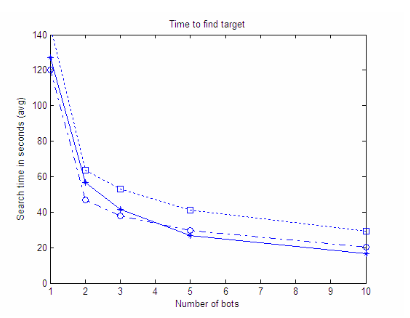
\includegraphics[scale=0.9]{Images/HerefordResults.png}
    \caption{dPSO Time to find Target \protect\cite{hereford_2006} }
    \label{fig:dPSO Time to find Target}
\end{figure}

\subsubsection{AGLDPSO}
In Wang et als. paper "Adaptive Granularity Learning Distributed Particle Swarm Optimization for Large-Scale Optimization" a distributed implementation is proposed, called AGLDPSO(Adaptive granularity learning distributed particle swarmoptimization) \cite{wang2020adaptive}. AGLDPSO uses a master-slave relationship when creating distributed particles, which is significantly different to Herefords distributed model, whereby all particles where peers within a swarm, there was no orchestration or master controller. Each particle, or robot was aware of all other robots in the swarm and updated accordingly. In AGLDPSO, a master acts as the intermediary and updates all particles in the population. This works very well for their implementation, but creates a network bottle neck that dSPO altogether avoids. When tested against multiple other optimisation algorithms the authors found that AGLDPSO "\textit{achieves a promising and satisfying performance when solving the large-scale optimization problems.}". 
\begin{figure}[H]
    \centering
    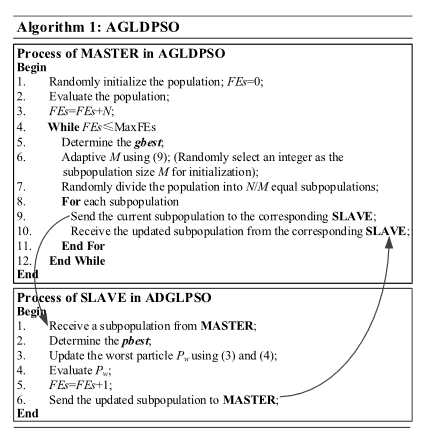
\includegraphics[scale=0.8]{Images/AGLDPSO.png}
    \caption{Flow Diagram of AGLDSPO \protect\cite{wang2020adaptive} }
    \label{fig:Flow Diagram of AGLDSPO}
\end{figure}

\section{Evaluating performance}
\subsection{Benchmarking}
Benchmarking, also referred to as "best practice benchmarking" or "process benchmarking", is  a  method  of  conducting  necessary  actions  and  activities  in  order  to evaluate  how  a  given  piece  of  software  or  a  system  is  going  to perform  once  it  is deployed and used in the field \cite{vokolos1998performance}. When speaking of software performance we general refer to throughput, stimulus, response time, or some combination of the two\cite{vokolos1998performance}.  It is also a way of assessing the system’s availability. Meaning that whenever the system undergoes high levels of stress, be it increasing the number of processed requests (throughput), or high resource consumption (machine resources), the system still processes these requests or events in acceptable numbers\cite{vokolos1998performance}.  Usually benchmarking involves predicting how a technology will behave once its used in regular every day life, for instance benchmarking a web server will allow organisations to predict how well it will cope with increased web traffic. The predictions allow organisation to anticipate potential limitations, and can lead the organisation to a plan to overcome those limitations. 

\subsection{Evaluating PSO performance}
 In literature PSO is often benchmarked against other variants of PSO,the original implementation of PSO, or some other optimisation algorithm. For example in the literature around AGLDPSO, it was bench marked against  the following algorithms; CCPSO2, SL-PSO, CSO, DMS-L-PSO, DSPLSO, DLLSO, DECC-DG, DECC-G, and MLCC \cite{wang2020adaptive}, half of which are PSO implementations. 
 % Need to finish this off. 
 
 
\section{Research Gaps}
As outlined above there has been a large amount of research in the area of Swarm intelligence over the past 20 years. We can see in J. F. Schutte et. al article they had a comprehensive cover of using parallel PSO \cite{schutte2004parallel}, however to limit network connection time the used a parallel processor for running the algorithm. This would certainly cut down on networking connection times, however it cant be described as truly a distributed algorithm. S. Burak Akat and Veysel Gazi focused much more on the distributed aspect of the algorithm, but no effort was made at running comparisons between the distributed version and a non distributed version of the algorithm \cite{akat_gazi_2008}. James M. Hereford again focused on the distributed aspect of the algorithm, with no relative benchmarks comparing it to a non distributed version. \cite{hereford_2006}

The gap identified for this article is the performance benefits of running a PSO algorithm in distributed environments vs centralised environments. As you can see above there has been plenty of research into crafting and testing distributed implementations of the PSO algorithm, but as far as I can find in my research there has been no comparison done of testing the PSO algorithm in distributed environments vs centralised environments and comparing the results.
%Needs another paragraph or two.

\section{Conclusion}


% Design and methodology chapter
% ============================================================= %
\chapter{Experiment design and methodology}
\section{Introduction}
This chapter presents the design used to craft the experiment and the methodologies used to test the results from that experiment. The chapter will cover the aim of the research, the design and implementation of the experiment, data output design and will conclude with design conclusions. 
\section{Aim of Research}
The aim of this paper is to find out if a point exists when scaling a PSO algorithm, that it becomes more efficient to run a a distributed algorithm instead of as a centralised algorithm. Increasing the number of active particles in a PSO algorithm can lead to a decline in performance, as for each iteration or epoch the machine must dedicate more and more power to recalculate particles positions and best evaluations. In a distributed model this burden can be divided across a number of machine, however in order to calculate global bests network communications must occur between machines in order to form the swarm. Network communications are inherently slower than local connection communications, however at high levels of active particles this speed decrease may be alleviated by the increased computational power available. 

\section{Hypothesis}
\subsubsection{Null Hypothesis H\textsubscript{0}:}
The time taken to find a stabilised result from using a distributed network of swarms never exceeds the time lost from the network communications needed to update swarms of each others presence and activities.

\subsubsection{Alternate Hypothesis H\textsubscript{1}:}
The increased speed to solution time from using a distributed network of swarms exceeds the time lost from the network communications needed to update swarms of each others presence and activities once the number of particles and/or swarms has reached a sufficient level.

\section{Design overview}
In order to create the data required to prove/disprove the hypothesis two code base's will need to be created. One code base will need to handle generating the data required for a centralised PSO,and the other will need to generate the data from a distributed PSO implementation. Each will need to be able to run the same fitness functions, and operate nearly identically except for the distributed implementation which will need to call other PSO nodes to run swarms rather than running them on the local system. 
The coded system will need to be run multiple times with the same inputs in order to account for the random element inherit in the PSO algorithm. After each run the system will need to output all generated data, and a data aggregator will need to sort, average and output all the data in order for it to be evaluated.

\begin{figure}[H]
    \centering
    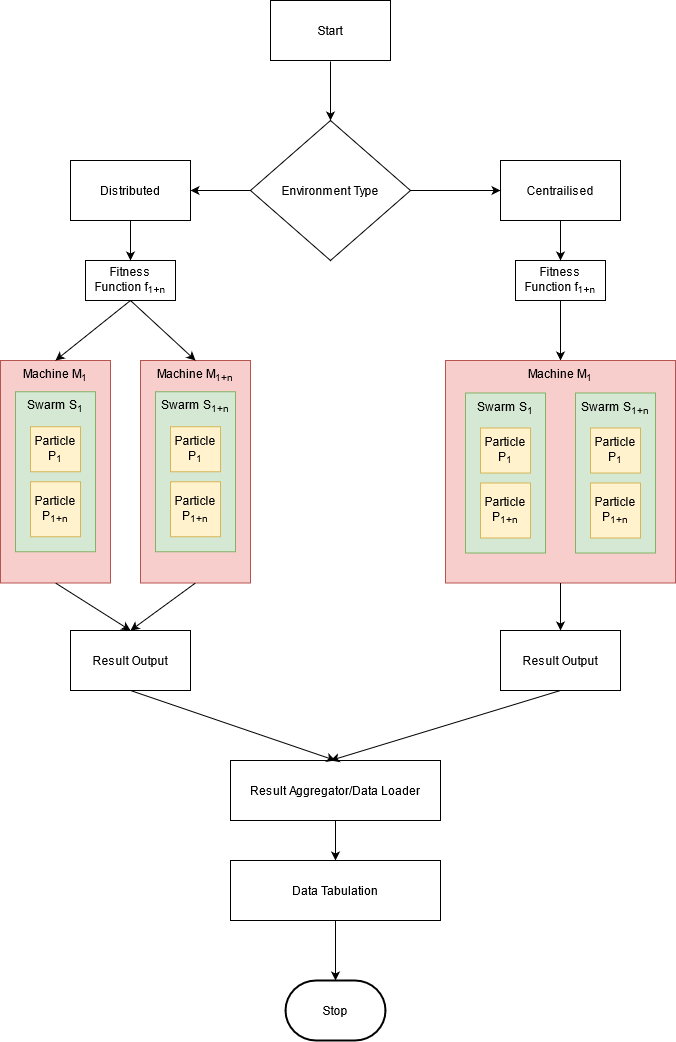
\includegraphics[scale=0.6]{Images/ExperimentFlow.png}
    \caption{Experiment Design Flow Chart}
    \label{fig:Experiment Design Flow Chart}
\end{figure}
Figure 3.1 displays the flow of the experiment. First the environment type will be chosen, then the from that point the require fitness function will be chosen. To give greater breath to the results four different fitness functions will be used, with varying degrees of complexity. Once the fitness function has been chosen, the swarms and particles can be initialised with the function implementation. In the case of the centralised implementation this will be the same machine, in the decentralised implementation swarm nodes will be contacted and initialised. Once each environment type has completed its run and found a stable answer the implementations will return a data response object. 

At this point the data aggregator will pull in the results from both implementations, with corresponding configuration details and generate a data output file useful for data comparison. This data file will be loaded into a data tabulation tool, whereby the results can be inspected and comparisons can be drawn up. At this point the study will be able to draw conclusions on whether the alternate hypothesis can be accepted or rejected.  

\subsection{Centralised PSO Design}
Expanding on the design overview, the centralised implementation will need to perform several steps in order to generate the required results set. Firstly it will initialise and create a parameterised number of swarms, each with a parameterised number of particles. At this point the first iteration will begin for all swarms. This will all occur on the one node. The iteration will follow the same format as what was discussed in section 2.2.1. Each swarm will attempt to find its group best value. All swarms will then report the group best value. At this point the controller class, which will also be the class that instantiates the swarms, will try and calculate if a "settled" group best value has been found. What this means is that at a certain point the algorithm will settle on a particular value, the global minimum. This will be the optimum solution to the fitness function. In this context settled means that for a certain number of iterations the same group best value will be returned. So the system will need to record past values and compare against returned values to see if the same value has been returned for multiple iterations in a row. When this has occurred the domain controller will calculate the time to arriving at this optimal solution, and the number of iterations it took to find that value. 
The basic flow of Centralised implementation is shown below. 
\begin{figure}[H]
    \centering
    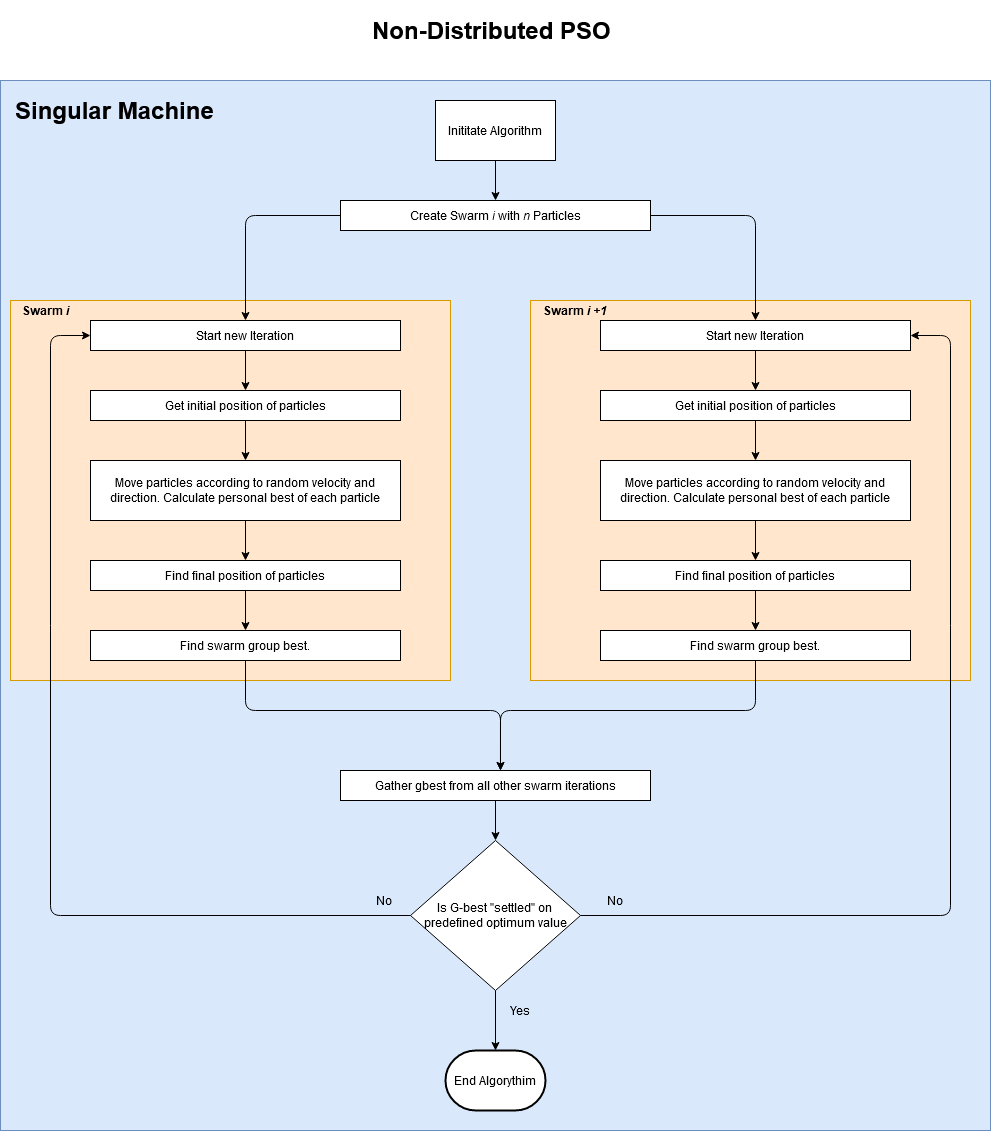
\includegraphics[scale=0.4]{Images/FlowDiagramNonDistibutedPSO.png}
    \caption{Flow Diagram of Centralised Particle Swarm Algorithm}
    \label{fig:Flow Diagram of Centralised Particle Swarm Algorithm}
\end{figure}

\subsection{Distributed PSO Design}
\begin{figure}[H]
    \centering
    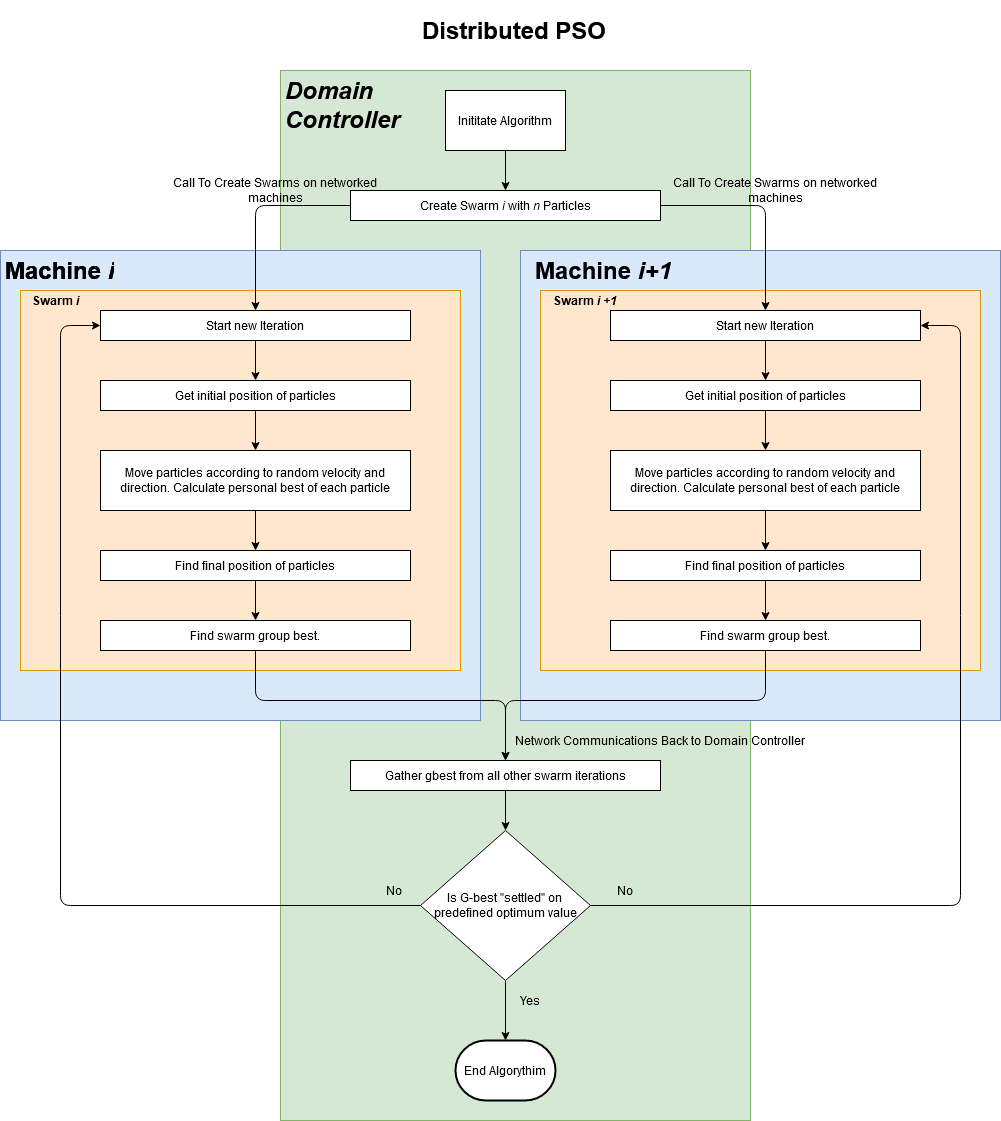
\includegraphics[scale=0.4]{Images/FlowDiagramDistibutedPSO.png}
    \caption{Flow Diagram of Distributed Particle Swarm Algorithm}
    \label{fig:Flow Diagram of Distributed Particle Swarm Algorithm}
\end{figure}
As discussed in the overview, the distributed implementation will function similarly to the centralised implementation to keep differences in results to a minimum. The only functional difference will be that swarms will be logically separated across multiple machines in the distributed implementation. Where the centralised implementation will be running a domain controller, and all swarm instances, the distributed implementation will feature a domain controller on a single node, calling out to other networked nodes, that will startup and iterate individual swarms with a parameterised number of particles. Once an iteration ends the node will communicate back to the domain controller, which will collect responses from all active swarms, and check to see if the swarms have "settled" on the parameterised global minimum value. 
If they have the domain will stop the nodes from running any further iterations, collect resulting values, ie. number of iterations and time to solution. Network time will be accounted for in the time to solution value.

\section{Distributed environment}
In order to create a distributed environment for the distributed implementation for this project a cloud provider was required. Using these cloud providers a virtual machine can be created and initialised, allowing the end user or developer to install custom software and applications. In this instance it allows the distributed implementation and centralised implementation to be deployed and run in a containerised environments. Snapshots where used to ensure consistency between the two implementations, and between the nodes of the distributed implementation. To facilitate this a number of different providers where considered, including AWS(Amazon Web Services), Google cloud and Digital Oceans. Each had a containerised virtual machine product that allowed the deployment of java applications, along with unique domain names and other internet connection utilities, however only one provider was required and Digital Ocean was chosen as the provider for this project. 

\subsection{DigitalOcean}
Digital Ocean is an Infrastructure as a Service(IaaS) platform for software developers. It allows developers to create containers in a simple and quick manner. To deploy Digital Ocean's IaaS environment, developers launch a virtual machine instance, which DigitalOcean calls a "droplet.". This is containerised, and a number of operating systems can be chosen to initialise the doplet. The OS's available to developer include: Ubuntu, CentOS, Debian, Fedora, CoreOS or FreeBSD. Digital ocean also offer the ability to choose the geographic region the droplet will be created in, and some other configuration options such as the amount of dedicated ram, number/quality of CPU, and the size of the on-board hard drive. Once initialised the developer may install their own custom software, or use some prepared packages from digital ocean to help speed along deployment. 

Once the droplet has been created developers have the ability to monitor activity from their browser using digital oceans control panel. They also have the ability to update the domain name, and create a VPN(Virtual Private Network) for the droplet. Snapshots of the droplet can be taken at any time and used to recreate it if required. Digital ocean is a very affordable option among its peers, with basic containers costing at minimum 0.00744\$ an hour, working out at 5\$ a month. For that price digital ocean provide a container with one gigabyte of RAM, one core CPU and twenty gigabytes of on-board storage.

\subsection{Container and Network Design}
As previously mentioned the distributed provider used for this project will be digital ocean. Utilizing the containerisation service previously mentioned, a number of droplets will be created. Droplets will contain the implementation code in order to act as a domain controller and as a swarm node. However each node will only ever act as a domain controller or a swarm node. This design can be seen in figure \ref{fig:ContainerDesignOverview}. When running the distributed implementation the domain controller node will be called using the same request as the non-distributed method, however instead of an integer defining the number of swarms to be used, a list of IP address will be passed in. These IP address will correspond with the IP address's for the droplets running swarm nodes. The domain controller will then connect with each of these droplets, initialise the swarm node with the passed in configuration values, begin iterating and collecting response from all connected swarm nodes.

\begin{figure}[H]
    \centering
    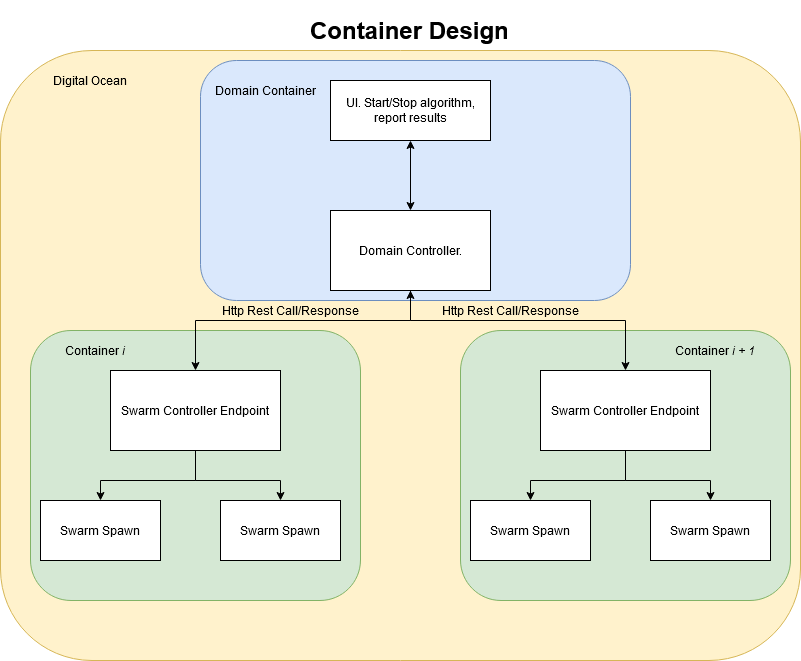
\includegraphics[scale=0.4]{Images/ContainerDesign.png}
    \caption{Container Design Overview}
    \label{fig:ContainerDesignOverview}
\end{figure}

This design does feature a core flaw in that it creates a central dependency in the domain controller, and if the domain controller is not sufficiently powerful enough it may also become a bottleneck. However in order to keep the results as consistent and in line with the centralised implementation, the domain controller will be the same droplet size as all other swarm nodes. 

\section{Data Design and Data Capture Overview}
For the purpose of this project the following variables will be recorded for comparison. 
\begin{table}[H]
  \centering
    \begin{tabular}{| c | c | c |}
    \hline
     & \textbf{Variable Description} & \textbf{Data Type} \\ \hline
    \textbf{Time} & Time taken to get to solution & Integer \\ \hline
    \textbf{N-Particles} & Number of active Particles  & Integer \\ \hline
    \textbf{N-Swarm} & Number of active Swarms. & Integer \\ \hline
    \textbf{Environment-Type} & Distributed or Centralised & String \\ \hline
    \textbf{Iterations} & Total number of iterations to reach a solution & Integer \\ \hline
    \textbf{finalGroupBest} & Final group best from all swarms & Integer \\ \hline
    \textbf{averageBestX} & Average best X value across all swarms  & Integer \\ \hline
    \textbf{averageBestY} & Average best Y value across all swarms & Integer \\ \hline
    \end{tabular}
  \caption{Data output variables}
  \label{tab:data_output_design}
\end{table}
Starting with the first variable in table 3.1, the time variable, this will represent the amount of time it took the specific test to calculate an answer. This will be recorded in milliseconds, and it will be calculated by the domain controller, starting from the time it initialise the swarms in either the distributed implementation or the centralised implementation, and ending when either implementation arrives at a settled answer. The number of particles and swarms will be specified in the request when running the algorithm, but will also be recorded as part of the output for ease of comparison of results. Again environment type will be specified in the request, and recorded in the output for comparison. The Iterations variable will be used to record the number of iterations or epochs it took to reach a settled solution. This will also include the defined number of iterations for a result to be considered settled, which will inflate the total number of iterations, however as this affects all test runs it will have no significant impact on the final values. Final group best will record the final solution answer. All iterations should come to the same value, as the fitness functions used will contain only one global minimum, however it was recorded to see if there was any variation in the results between implementation types. Similarly with average best x and y all implementations types should conclude with the same values, but they where recorded to see if there was any variation.
This data will be outputted to a JSON(JavaScript Object Notation) file at the end of each test run. The JSON file will be named in the following convention:

\verb|<Function-Name>_<SwarmNumber>_<ParticleNumber>.results.json|


\subsection{Data Aggregation}
As mentioned in section 3.4 Design overview, due to the random element of the PSO algorithm, an average of results with the same parameters will need to be taken. Therefore multiple data output files will be generated for tests with the same inputs. In combination with multiple tests with varied numbers of particles and swarms, a large number of output files will be generated. To deal with this a data aggregation system will need to be created. This aggregation system will load in results with the same input variables, create an average values for the time to solution variable, number of iterations, finalGroupBest, and averageBestX/Y values. Values will then be outputted  into a single data file, with results from the distributed an centralised implementation being directly compared.

\section{Design and Methodology Summary}
This chapter presented an overview of the design and methodology used for this research. It discussed the overarching design of the experiment, with subsequent sections going into a more detailed design of specific elements of the research. Data output and capture was also discussed, with a data output design presented in some detail. 

% Experiment Implementation details(The only fun chapter really) 
% ============================================================= %
\chapter{Experiment Implementation}

\section{Introduction}
This chapter will expand on the previous chapter and cover the implementation details in more depth. Coding examples will be provided for more clarity on how the two PSO implementations function. Additionally the test harness and data loader that where created for this experiment will be expanded upon and coded examples of each will be given.

\section{PSO Implementations}

\subsection{Java}
For the purpose of this study java will be used as the implementation language. Java is a mature language, with its initial 1.0 release in 1995. Since then its gone through multiple iterations and major version changes. It has been largely adopted by large enterprise organisations due to its stability and feature rich ecosystem. Java was chosen due to the "deploy anywhere" model that allows for applications to be run on any operating system that supports a JVM(Java Virtual Machine). This will be a large benefit when the application is deployed to a distributed environment. Other advantages of using Java are its quite performant, has a large set of supported libraries and extensions, along with a very active community and a wide range of supporting tools and documentation.

\subsection{Spring Boot}
Spring Boot is an open source Java-based framework, that includes many utilities and libraries that allows a developer to quickly create a "production-grade"\footnote{https://spring.io/projects/spring-boot} application and is developed by Pivotal team. Spring boot is configured with an embedded servlet container, contains many auto-configurations features for ease of development, and provides plenty of additional tools for crafting microservices. 

Spring boot was used in this experiment because of its mature and stable nature, and the ability to easily create REST(Representational state transfer) based microservices. Due to the distributed nature of the experiment, REST API calls where used to facilitate the messaging between swarm nodes and the domain controller. More on this will be discussed in the following sections. Spring boot allows developers to quickly configure REST API's, and is reasonable performant during runtime \footnote{https://spring.io/blog/2018/12/12/how-fast-is-spring}. Spring boot also allows developers to easily configure a number of different logging tools and frameworks to aid in debugging runtime errors and exceptions.

\subsection{Centralised Implementation}
Using spring boot a basic rest controller was created, whereby the swarm 
\begin{lstlisting}[language=Java]
@RestController
public class CentralisedController {
    @Autowired
    private NonDistributedService nonDistributedService;

    @PostMapping("/runSwarm")
    public Response runNonDistributedSwarm(@RequestBody Request request) throws Exception {
        return nonDistributedService.runMultiSwarm(request);
    }
}
\end{lstlisting}
\captionof{lstlisting}{Centralised Rest Controller}

\subsection{Distributed Implementation}

\subsection{Fitness Functions overview}

\section{Test Harness}

\subsection{Postman/Newman and NodeJs}

\subsection{Implementation}

\section{Data aggregator implementation}

\section{Implementation conclusion}


% Results, evaluation and discussion chapter 
% ============================================================= %
\chapter{Results, evaluation and discussion}
\section{Introduction}

\subsection{Centralised results}

\subsection{Distributed results}

\section{Performance comparison}

\section{Network and other environment variations and impact}

\section{Conclusions}

\subsection{Metrics}



% Concluding chapter
% ============================================================= %
\chapter{Conclusion}
\section{Research Overview}
\section{Problem Definition}
\section{Design/Experimentation, Evaluation \& Results}
\section{Contributions and impact}
\section{Future Work \& recommendations}


% End of thesis content
% ============================================================= %

% Include the bibligraphy by referencing the correct .bib file
\bibliography{main_bibliography}

% Optional appendices
\appendix
\chapter{}
Listing A.1 shows and example data output produced for the booths fitness function from a distributed and centralised PSO implementation. 
\begin{lstlisting}
{
	"finalGroupBest": 0.0,
	"averageBestX": 1.0000000000000003,
	"averageBestY": 3.0,
	"iterations": 151,
	"timeToSolution": 1303,
	"resultsList": [
		{
			"swarmId": 0,
			"machineIpAddress": "138.68.142.96",
			"results": [
				{
					"step": 0,
					"best": 20.288124656313526,
					"bestPositionX": 0.0,
					"bestPositionY": 0.0
				}
				.....
		}
	]
}
\end{lstlisting}
\captionof{lstlisting}{Data output example}

\end{document}